\chapter{Análisis de Resultados}
\section{Capturas del programa en ejecución}
\\
A continuación se presenta en orden el proceso de ejecución del programa con una n $=$ 8,
donde iremos mostrando capturas de pantalla de todo el proceso, posteriormente a esto, 
indicaremos al programa que queremos otra $n$, que en este caso, será una $(n)$ aleatoria.

\begin{enumerate}
\item Iniciamos el programa, donde nos pregunta en un pequeño menú si queremos que introduzcamos la $"$n$"$ manualmente o aleatoriamente. Para el caso de ejemplo y de manera que se pueda visualizar digitaremos la opción 1 en el menú para posteriormente digitar que se construya un palíndromo de longitud 8. Podemos ver que al finalizar al cabo de milisegundos nos muestra un mensaje que nos indica donde están los archivos de salida, donde se guardó la construcción. Observar figura 2.1\newline


\begin{figure}[h]
\begin{minipage}{0.3\textwidth}
    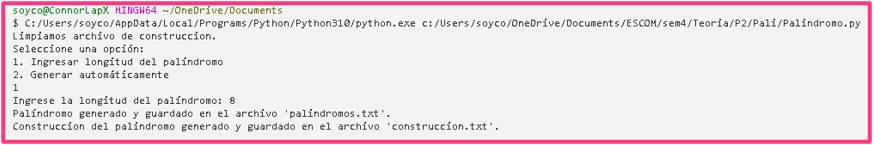
\includegraphics[width=4\linewidth]{Images/1.png}
\end{minipage}
\caption{Inicio del programa para n=8.}
\label{fig:imagen}
\end{figure}
\newpage
\item Aquí se puede apreciar el archivo de palindormo.txt, donde es en el dónde podemos apreciar el palíndromo resultante de la producción, al igual que podemos ver la longitud ingresada por el usuario.
Observar la Figura 2.2.\newline
\begin{figure}[h]
\begin{minipage}{0.3\textwidth}
    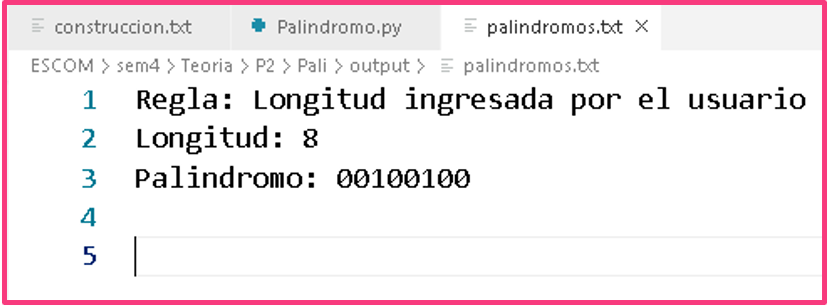
\includegraphics[width=4\linewidth]{Images/2.png}
\end{minipage}
\caption{Archivo de salida $"$palindormo.txt.$"$}
\label{fig:imagen}
\end{figure}

\item Aquí se puede apreciar el archivo de salida de construccion.txt, donde es en el dónde podemos apreciar la construcción paso a paso del palíndromo según la longitud registrada manual o aleatoriamente. Podemos observar el paso en que vamos y la regla que se aplicó y el resultado de la producción en la que vamos. Observar la Figura 2.3.
\newpage
\begin{figure}[h]
\begin{minipage}{0.3\textwidth}
    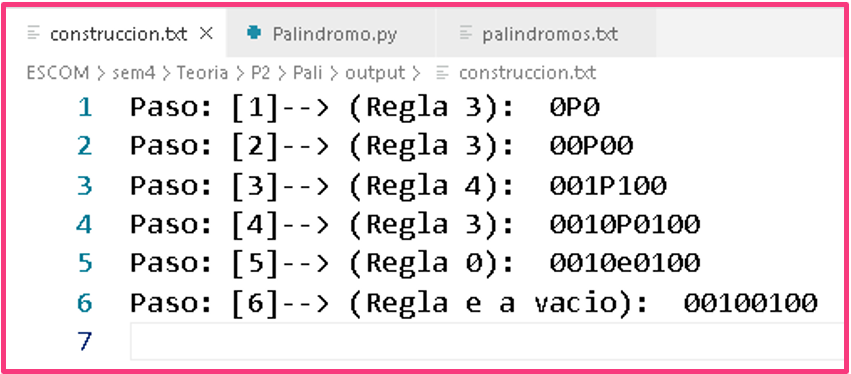
\includegraphics[width=4\linewidth]{Images/3.png}
\end{minipage}
\caption{Archivo de salida $"$construccion.txt.$"$}
\label{fig:imagen}
\end{figure}

\item Para el caso de ejemplo y de manera que se pueda visualizar digitaremos la opción 2 en el menú para posteriormente dejar que se construya un palíndromo de longitud aleatoria. Podemos ver que al finalizar al cabo de milisegundos nos muestra un mensaje que nos indica donde están los archivos de salida, donde se guardó la construcción. Observar la Figura 2.4.
\begin{figure}[h]
\begin{minipage}{0.3\textwidth}
    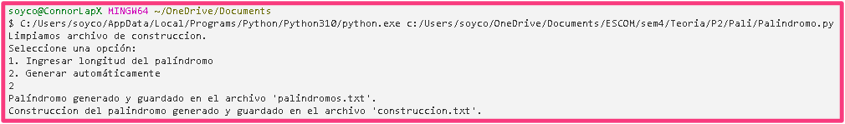
\includegraphics[width=4\linewidth]{Images/4.png}
\end{minipage}
\caption{Inicio del programa para n aleatoria.}
\label{fig:imagen}
\end{figure}
\newpage
\item Aquí se puede apreciar el archivo de palindormo.txt, donde es en el dónde podemos apreciar el palíndromo resultante de la producción, al igual que podemos ver la longitud registrada aleatoriamente. Observar la Figura 2.5.
\begin{figure}[h]
\begin{minipage}{0.3\textwidth}
    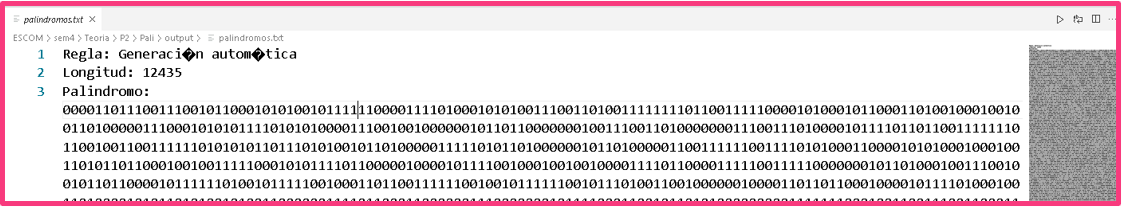
\includegraphics[width=4\linewidth]{Images/5.png}
\end{minipage}
\caption{Archivo de salida $"$palindormo.txt.$"$}
\label{fig:imagen}
\end{figure}

\item Aquí se puede apreciar el archivo de salida de construccion.txt, donde es en el dónde podemos apreciar la construcción paso a paso del palíndromo según la longitud registrada manual o aleatoriamente. Podemos observar el paso en que vamos y la regla que se aplicó y el resultado de la producción en la que vamos. Observar la Figura 2.6.
\begin{figure}[h]
\begin{minipage}{0.3\textwidth}
    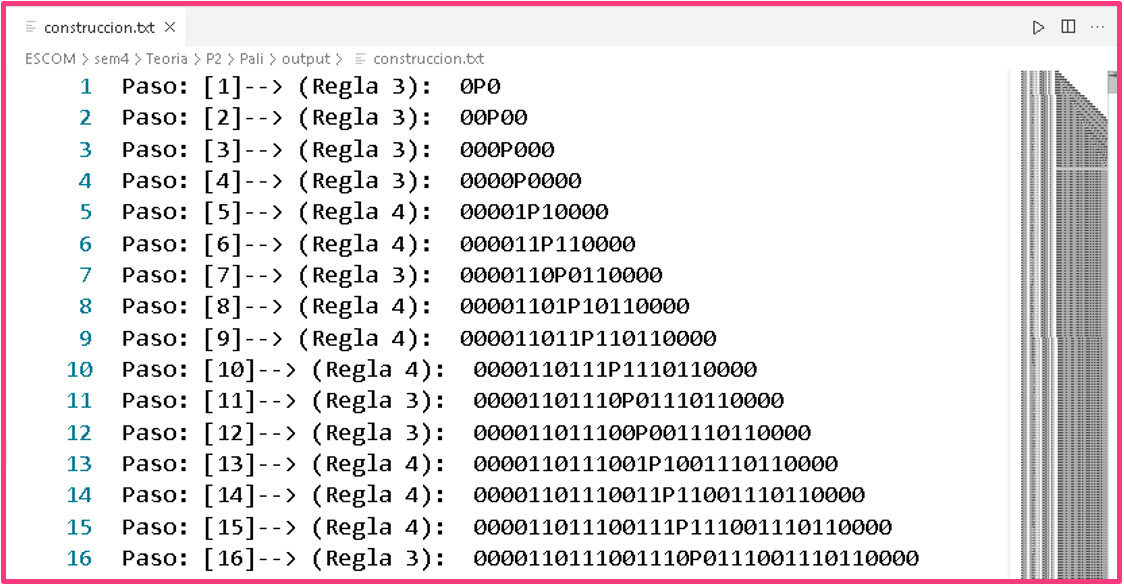
\includegraphics[width=4\linewidth]{Images/6.png}
\end{minipage}
\caption{Archivo de salida $"$construccion.txt.$"$}
\label{fig:imagen}
\end{figure}
